\documentclass[11pt]{article}
\usepackage [french]{babel}
\usepackage [T1]{fontenc}

\usepackage[linesnumbered, ruled, french, onelanguage]{algorithm2e}
\usepackage{adjustbox}%Permet de centrer les figures dans la largeur de la page même si les figures sont plus larges que \textwidth
\usepackage{amssymb}
\usepackage{amsmath}
\usepackage[toc,page,title,titletoc,header]{appendix}
\usepackage{expl3}%Pour la control sequence /ExlpSyntaxOn demandée par l'utilisation de subfiles apparemment...
\usepackage{gensymb}%pour pouvoir écrire le signe °
\usepackage{geometry}%Pour changer la largeur des marges du document notamment
\usepackage{graphicx}
\usepackage{hyperref}%pour les liens dans la bibliographie
\usepackage{listings}
\usepackage{placeins}%pour utiliser FloatBarrier afin que les figure respectent bien leur position dans le code
\usepackage{slashbox}%Case séparée en deux tout en haut à gauche des tableaux à double entrées
\usepackage{stmaryrd}%pour les crochets à double barres d'intervalles de nombre entiers
\usepackage{tikz}
\usepackage{xcolor}%/definecolor et /color
\usepackage{subfiles}

\usepackage{etoolbox}%pour /AtBeginEnvironment
\AtBeginEnvironment{appendices}{\renewcommand{\thesection}{\Alph {section}}}%Pour recommencer à compter les sections à 0 en rentrant dans l'annexe et pour compter avec des lettres et non des chiffres
\renewcommand{\appendixpagename}{\centering Annexes}%Pour centrer le titre de la partie annexe
\renewcommand{\appendixtocname}{Table des annexes} % Pour faire apparaître les annexes dans la table of contents

%%%%%%%%%%%%%% Couleurs de: https://texblog.org/2011/06/11/latex-syntax-highlighting-examples/ %%%%%%%%%%%%%%
\definecolor{javared}{rgb}{0.6,0,0} % for strings
\definecolor{javagreen}{rgb}{0.25,0.5,0.35} % comments
\definecolor{javapurple}{rgb}{0.5,0,0.35} % keywords
\definecolor{javadocblue}{rgb}{0.25,0.35,0.75} % javadoc
 
\lstset
{
language=Java,
keywordstyle=\color{javapurple}\bfseries,
stringstyle=\color{javared},
commentstyle=\color{javagreen},
morecomment=[s][\color{javadocblue}]{/**}{*/},
numbers=left,
numberstyle=\tiny\color{black},
stepnumber=1,
numbersep=10pt,
tabsize=4,
showspaces=false,
showstringspaces=false}
%%%%%%%%%%%%%% Couleurs de: https://texblog.org/2011/06/11/latex-syntax-highlighting-examples/ %%%%%%%%%%%%%%





\author{}
\title{Ray-Tracer}
\date{}
\geometry{hmargin=3cm, vmargin=2cm}

\begin{document}
\tableofcontents
\newpage

\maketitle

\section{Détail des parties techniques}
\subsection{Le Ray Tracer}
\subsubsection{L'algorithme de base}
\label{rayTracingBase}

\subfile{latex/RT/algoBase.tex}

\subsubsection{L'ombrage de Phong}
\label{ombragePhong}

\subfile{latex/RT/ombragePhong.tex}

\subsubsection{Les réflexions}

\subfile{latex/RT/reflections.tex}

\subsubsection{Les réfractions}
\label{refractions}

\subsubsection{Le damier et le ciel (skybox)}
\label{checkerboardSkybox}

\subfile{latex/RT/checkerboardSkybox.tex}

\subsection{Le multithreading}

\subfile{latex/RT/multithreading.tex}

\subsection{Les mouvements de caméra}
\label{mouvementsCamera}

\subfile{latex/RT/mouvementsCam.tex}

\section{Structuration du projet}
\subsection{Les packages}
\subsubsection{Liés au Ray Tracer}

\subfile{latex/packages/RTpackages.tex}

\subsubsection{Le package materials}

\subfile{latex/packages/materials.tex}

\section{Mesures de performance}

\subfile{latex/other/mesuresPerf.tex}






\newpage%Nouvelle page pour les annexes
\begin{appendices}
	\section{Le ray tracer}
		\subsection{Configuration d'une caméra, d'une scène et de rayons}
		\begin{figure}[h!]
			\adjustbox{center}{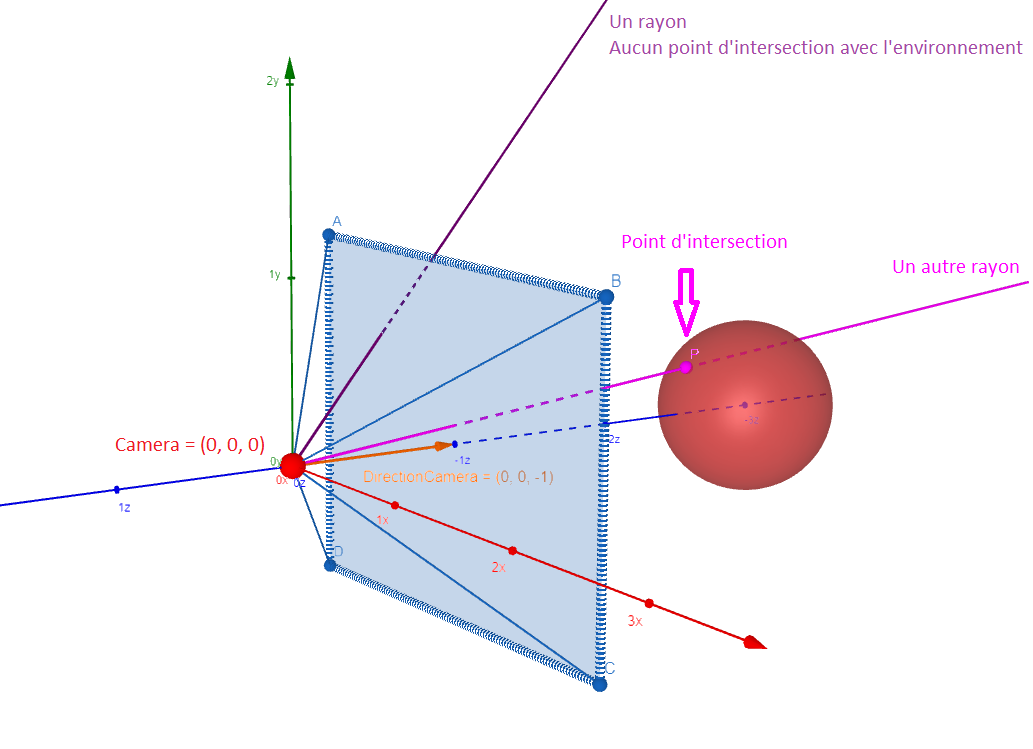
\includegraphics[width=1.1\textwidth]{img/rt/repCam2Rayonsv2.png}}
		
			\caption{Des rayons sont tirés depuis la caméra dans sa direction de regard. Nous cherchons les points d'intersection avec les objets de la scène}
		\end{figure}
		\FloatBarrier
		\label{annexe:repreCamRayon}

		\subsection{Le principe récursif des réflexions}
		\begin{figure}[!h]
			\adjustbox{center}{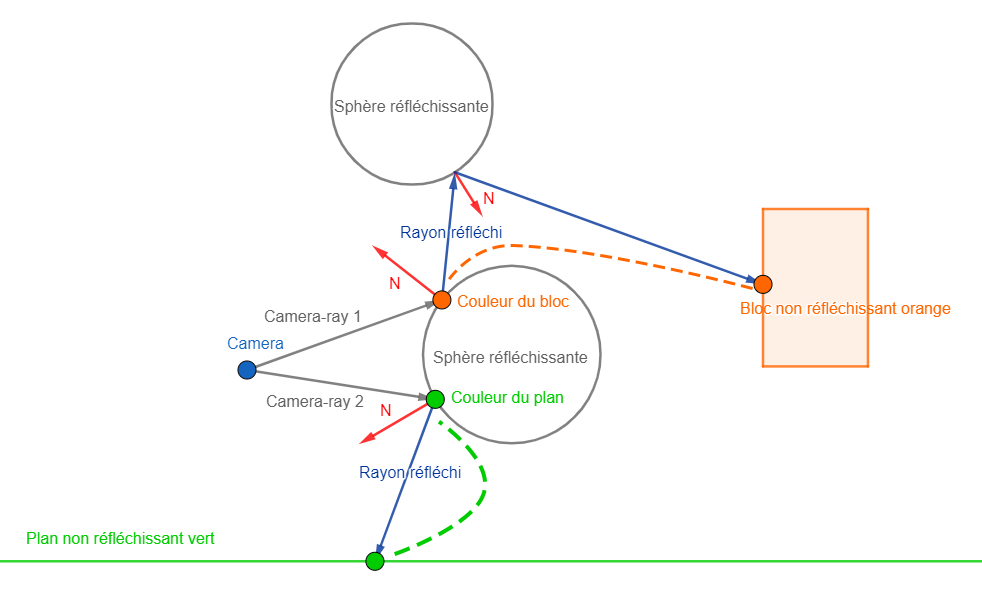
\includegraphics[width=1.1\textwidth]{img/rt/reflectionsSchema.png}}
		
			\caption{Exemple de rebonds successifs des rayons jusqu'à un objet non réfléchissant}
			\label{reflectionsSchema}
		\end{figure}
		\FloatBarrier
		\label{annexe:reflexionsRecursives}
\FloatBarrier
\end{appendices}

\newpage%Nouvelle page pour la bibliographie
\nocite{*}
\bibliographystyle{unsrt}
\bibliography{bibliography/sources}

\end{document}